\documentclass{article}
\usepackage[utf8]{inputenc}
\usepackage[russian]{babel}
\usepackage{graphicx}
\usepackage{amsmath}
\usepackage{breqn}
\usepackage{wrapfig}
\usepackage{float}
\usepackage{multirow}
\usepackage{caption}
\usepackage{subcaption}

\graphicspath{ {./data/images} }
\author{Александр Романов Б01-107}
\date{}
\title{4.4.1 Изучение амплитудной решётки}

\begin{document}
\maketitle
\section{Введение}
\subsection{Цель работы}
Знакомство с работой и настройкой гониометра Г5, определение спектральных характеристик амплитудной решётки.
\subsection{В работе используются}
Гониометр, дифракционная решётка, ртутная лампа.
\section{Работа}
Проведём юстировку системы, руководствуясь правилами, изложенными в Приложении.
Характеристики установки:
\[ d = 1/ 500\; mm = 0.002\; mm = 2\cdot 10^{-6}\; m \]

\begin{figure}[H]
  \centering
  \begin{tabular}{|c|c|c|c|c|c|c|c|c|}
    \hline
    \textnumero & 1 & 2 & 3 & 4 & 5 & 6 & 7 & 8 \\\hline
    \(\lambda, \; nm\) & 690.7 & 623.4 & 579.1 & 577.0 & 546.1 & 491.6 & 435.8 & 404.7\\\hline
    Цвет & красн. & красн. & жёлт. & жёлт. & зелён. & голуб. & синий. & фиолет. \\\hline
    Яркость & 4 & 4 & 10 & 8 & 10 & 4 & 4 & 3\\\hline
  \end{tabular}
  \caption{Характеристики спектра ртутной лампы}
\end{figure}

\subsection{Установка решётки}
Установим решётку на столик так, чтобы её плоскость была перпендикулярна оси зрительной трубы и параллельна
одному из установочных винтов 8. В центре поля зрения будет расположена белая ахроматическая полоса
(спектр нулевого порядка). Высота полосы занимает менее четверти поля зрения трубы.

Винтом 8, перпендикулярным плоскости решётки, установим изображение щели в центр поля зрения. Отводя алидаду
в сторону от коллиматора, найдём в трубе спектр самого дальнего порядка и винтом 8, параллельным плоскости
решётки, снова приведём изображение щели в центр. Убедимся что при повороте трубы изображение щели и спектр
уходят не более чем на треть радиуса поля зрения.

\subsection{Исследование спектра ртутной лампы}
Подберём ширину входной щели коллиматора так, чтобы ширина линий жёлтого дублета была чуть больше промежутка
между линиями двойного штриха окуляра зрительной трубы. Установим удобную для наблюдения высоту щели.

Убедимся в справедливости формулы
\[ d\;sin\varphi \simeq \lambda \]
Для этого определим углы дифракции для двух ярких линий спектра (синего и зелёного) в одном порядке.

\[ \varphi_{b} = 12^{\circ}32'29'' \]
\[ \varphi_{g} = 15^{\circ}46'53'' \]

\textbf{Для синего:}
\[ d \; sin\varphi_{b} = 2\cdot 10^{-6} \cdot 0.217 \simeq 434\; nm  \]
Что точно совпадает с табличным значением длины волны для синего света (\(\lambda = 435.8\; nm\)).

\textbf{Для зелёного:}
\[ d \; sin\varphi_{g} = 2\cdot 10^{-6} \cdot 0.272 \simeq 544\; nm  \]
Что точно совпадает с табличным значением длины волны для зелёного света (\(\lambda = 546.1\; nm\)).

Измерим угловые координаты спектральных линий ртути в \(\pm 1\) порядках. Голубой свет: 
\[ \varphi_{blue0} = 14^{\circ}10'41'' \]
\[ \varphi_{blue1} = 14^{\circ}18'19'' \]

Для оценки угловой дисперсии решётки определим угловые координаты линий жёлтой пары во всех видимых
порядках спектра.
\[ \varphi_{y0} = 16^{\circ}41'36'' \]
\[ \varphi_{y1} = 16^{\circ}45'8'' \]
\[ \varphi_{y2} = 16^{\circ}47'51'' \]

Отсюда разность длин волн жёлтой пары:
\[ \delta\lambda_{yel} = 2\cdot 10^{-7} \cdot (0.288 - 0.287) = 2\; nm \]

Для определения аппаратной разрешающей способности (решётка + ганиометр + глаз) измерим угловую ширину
одной из линий жёлтой пары(по нулям интенсивности) в нескольких порядках.
\[ \Delta\varphi = 16^{\circ}42'2'' - 16 ^{\circ}41'30'' = 0^{\circ} 1'28'' \]

Для качественного определения аппаратной разрешающей способности \(R\) измерим расстояние между центрами
жёлтых линий.
\[ \delta\varphi = 0^{\circ}4'28'' \]

\subsection{Зависимость разрешающей силы от ширины пучка}
Настроим зрительную трубу на жёлтую пару. Определим начала отсчёта дополнительной щели с микрометрическим
винтом (момент её открытия) Получим:
\[ d_0 = 26\; \mu m \]
Откроем щель пошире и укрепим её на коллиматорном объективе. Уменьшая ширину щели, добьёмся предельного
разрешения жёлтой пары и запишем показания микрометрического винта:
\[ d = 300\; \mu m \]

\subsection{Обработка результатов}
Сведём результаты измерения углов дифракции для разных длин волн:
\begin{figure}[H]
  \centering
  \begin{tabular}{|c|c|c|c|c|}
    \hline
    \(\lambda, \; nm\) & 579.1 & 546.1 & 491.6 & 435.8 \\\hline
    \(\varphi\) & \( 16^{\circ}41'36'' \) & \( 15^{\circ}46'53'' \) & \( 14^{\circ}10'41'' \) & \( 12^{\circ}32'29'' \) \\\hline
  \end{tabular}
  \caption{Углы дифракции}
\end{figure}

Построим график:
\begin{figure}[H]
  \centering
  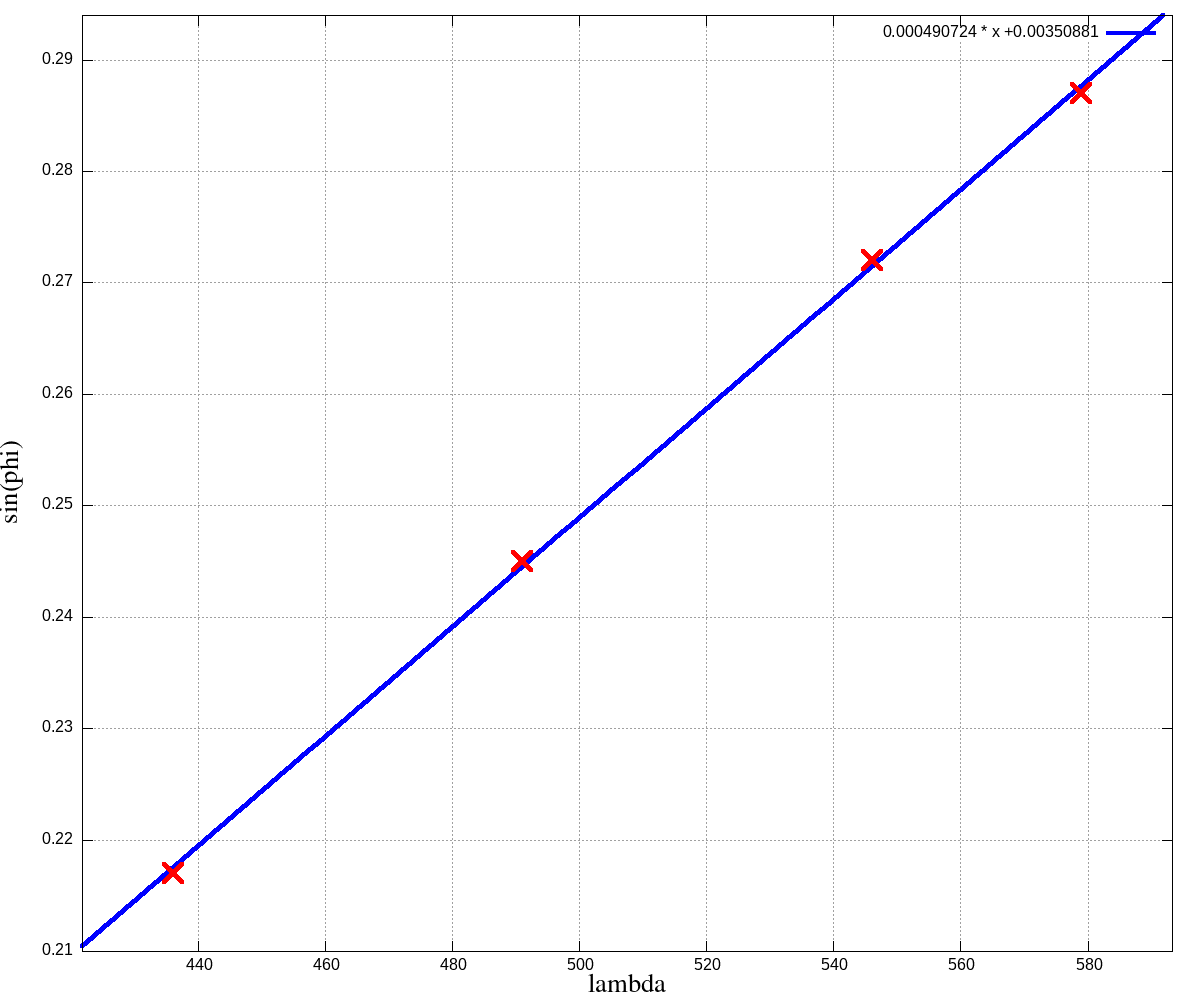
\includegraphics[width=0.8\textwidth]{sin.png}
\end{figure}

Результаты опроксимации вида (\(y = kx\)):
\[ k = (491 \pm 5)\cdot \; mm^{-1} \]

Т.е. экспериментально получена плотность решётки \(491 \pm 5\) штрих/m. Что достаточно точно совпадает
с теоретическим значением (\(500\) штрих/mm).


По измерениям координаты и угловой ширины жёлтой линии расчитаем экспериментальное значение
разрешающей способности:
\[ R = \frac{\lambda}{\Delta\lambda} = \frac{574\cdot 10^{-9}}{20\cdot 10^{-10}} \simeq 287  \]

Определим число эффективно работающих штрихов:
\[ N = \frac{R}{m} = \frac{287}{3} = 95 \]

\section{Выводы}
В ходе лабораторной работы:
\begin{enumerate}
  \item Были экспериментально измерены длины волн спектра ртутной лампы по их дифракционному углу.
  Результаты совпадают с теоретическими очень точно:
  \[ \lambda_{\text{синий}} = 434\; nm \; \text{vs}\;  436\; nm \]
  \[ \lambda_{\text{голубой}} = 489\; nm\; \text{vs}\;  491\; nm \]
  \[ \lambda_{\text{зелёный}} = 544\; nm\; \text{vs}\;546\; nm \]
  \[ \lambda_{\text{жёлтый}} = 573\; nm\; \text{vs}\;579\; nm \]
  \item Была экспериментально измерена разрешающая способность системы:
  \[ R = 287 \]
  \item Было определено кол-во активно работающих штрихов:
  \item Было экспериментально получена характеристика решётки:
  \[ 491\; \text{штрихов/mm} \; \text{vs}\; 500\; \text{штрихов/mm}\]
\end{enumerate}
\end{document}